%% ECSE 420 -- Project proposal

%
\documentclass[journal]{IEEEtran}
%
% If IEEEtran.cls has not been installed into the LaTeX system files,
% manually specify the path to it like:
% \documentclass[conference]{../sty/IEEEtran}


%My packages
\usepackage{graphicx,dblfloatfix}
\graphicspath{{./figures/}}
\usepackage[xetex,colorlinks=true,urlcolor = black, 
linkcolor=black,citecolor=black]{hyperref}


% correct bad hyphenation here
\hyphenation{op-tical net-works semi-conduc-tor}


\begin{document}

% paper title
% can use linebreaks \\ within to get better formatting as desired
\title{ECSE 548: Modified 8-bit Booth Multiplier}
%\author{\IEEEauthorblockN{Marco Kassis\IEEEauthorrefmark{1},
%Aryan Mojtahedi\IEEEauthorrefmark{1},
%Dimitrios Stamoulis\IEEEauthorrefmark{1} and
%Louis-Charles Trudeau\IEEEauthorrefmark{1}\IEEEauthorrefmark{2}}
%\IEEEauthorblockA{\IEEEauthorrefmark{1}McGill University, Montreal, Canada ~~~~~ \IEEEauthorrefmark{2}Ecole de technologie superieure, Montreal, Canada}
\author{\IEEEauthorblockN{Marco Kassis,
Aryan Mojtahedi,
Dimitrios Stamoulis and
Louis-Charles Trudeau}\\
\IEEEauthorblockA{Department of Electrical and Computer Engineering, McGill University, Montreal, Canada}
}

\markboth{ECSE 548, Introduction to VLSI - Final Report, December~03,~2013}%
{ECSE 548, Introduction to VLSI - Final Report, December~03,~2013}

% make the title area
\maketitle
\IEEEpeerreviewmaketitle


\graphicspath{ {./figures/} }


\begin{abstract}
%\boldmath
A Multiplier is one of the most important elements of any modern processor, whether it be for the sake of pure multiplication to evaluate for arithmetic purposes or for other functions that make use of that function. It is one of the processes that consume a significant amount of processing time, since it is a series of additions, making it very important to optimize. This report presents the modified booth algorithm applied on an 8-bit level. The multiplier’s performance is then compared to that of the Baugh-Wooley Multiplier with respect to area, transistor count and delay. Integration within the MIPS core is also implemented and presented in this paper. The CAD tool used for the design process is Electric, while testbenching was done by Verilog file exports on ModelSim, while the test vectors were generated using a C program.
\end{abstract}


% Note that keywords are not normally used for peerreview papers.

\begin{IEEEkeywords}
Multiplier; Modified Booth Algorithm; MIPS; Baugh-Wooley Multiplier.
\end{IEEEkeywords}



\section{Introduction}
\IEEEPARstart{T}{he} 
multiplication of 2 given 8-bit vectors, M and N, results in a vector larger than both of them, namely 16-bits. To regularly perform this multiplication, it has to be done bitwise, generating N partial products of the same size as M, shifted and then added to compute the value of the multiple.

Accordingly, using the most basic form of the array multiplier, we realize that that the most significant bit (MSB) takes 2M-2 time units till it reaches its final output. This is a significant waste of processing time, given that the multiplier is essentially on module within the entire processor. Hence, a logical optimization is to group the partial products together to reduce their number, hence reducing the number of additions that need to be done, which would reduce the amount of time taken to compute the product.

Modified booth algorithm introduces this type of grouping based on the inputs being inserted into the multiplier, which is discussed in the upcoming Section.
\emph{Our goal is to produce a fast 8-bit multiplier, reducing both area and time delay compared to the regular Baugh-Wooley Multiplier. The multiplier implements the ModifiedBooth Logic and is integrated within the reduced 8-bit MIPS processor.
}

\section{Booth Logic}

The booth logic depends on an important metric r, which defines the number of partial products to be grouped together. Accordingly, the radix of the system is defined to be 2r. The radix itself defines the weight by which each and every of the partial products differ from the one to the following. We hence observe that the weight of the r=2, is a radix of 4, since grouping together 2 elements will result in a shift of 2 between each of the partial products which is equivalent to multiplying by 4 from one to the following. The utilization of a radix-4 system provides a reduction in the number of partial products reaching $\frac{M+1}{2}$
instead of M, which is almost half, hence a significant improvement. The size of each vector is N+1.

The radix-4 system is the one used in this project. The 2 vectors being multiplied will be referred to as X and Y for convenience within this Section. This leads to having the 4 possible values of the partial products of Y being 0, Y, 2Y and 3Y. 2Y can be easily achieved using the single shift of the partial product; however, 3Y would require an adder, eliminating the whole point of the booth logic. Accordingly, a workaround would be to consider 3Y as –Y+4Y, while 2Y would become -2Y+4Y, with the first part of the sum accounted for earlier then the second part following that. This leads to observing of 3 bits at a time, the MSB from the previous subvector taken, with the other current 2. Accordingly Table\ref{tab:t1} shows the truth table for this type of implementation.

\begin{table}[!h]
%% increase table row spacing, adjust to taste
\renewcommand{\arraystretch}{1.2}
% if using array.sty, it might be a good idea to tweak the value of
% \extrarowheight as needed to properly center the text within the cells
\caption{Booth Logic - Truth Table}
\label{tab:t1}
\centering
%% Some packages, such as MDW tools, offer better commands for making tables
%% than the plain LaTeX2e tabular which is used here.
\begin{tabular}{| c | c | c | c | c | c | c |}
\hline
$x_{2i+1}$ & $x_{2i}$  &  $x_{2i-1}$ & $PP_{i}$ & $SINGLE_{i}$ &
$DOUBLE_{i}$ & $NEG_{i}$\\\hline
0 & 0 & 0 & 0 & 0 & 0 & 0\\\hline
0 & 0 & 1 & Y & 1 & 0 & 0\\\hline
0 & 1 & 0 & Y & 1 & 0 & 0\\\hline
0 & 1 & 1 & 2Y & 0 & 1 & 0\\\hline
1 & 0 & 0 & -2Y & 0 & 1 & 1\\\hline
1 & 0 & 1 & -Y & 1 & 0 & 1\\\hline
1 & 1 & 0 & -Y & 1 & 0 & 1\\\hline
1 & 1 & 1 & -0 & 0 & 0 & 1\\\hline
\end{tabular}
\end{table}


%\begin{figure}[h!]
%  \centering
%  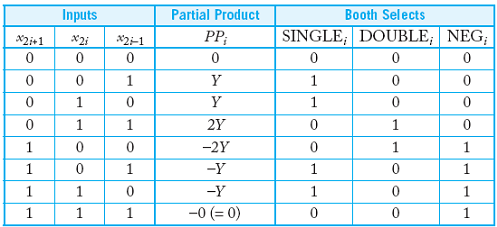
\includegraphics[width=0.35\textwidth]{1.png}
%  \centering
%  \caption{Booth Logic - Truth Table}
%  \label{fig:1}
%\end{figure}

The single, double and negative signals are the selected values that signify the operation to be implemented, which is elaborated on in the encoder part of next Section. The dot diagram with sign extension is seen in Figure
\ref{fig:2}.

\begin{figure}[h!]
  \centering
  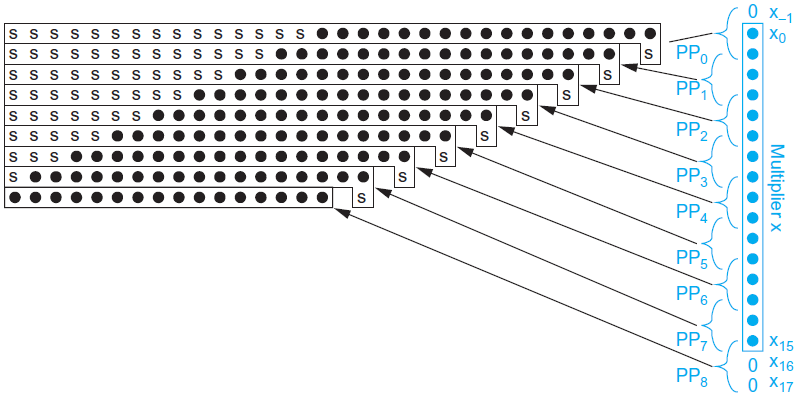
\includegraphics[width=0.4\textwidth]{2.png}
  \centering
  \caption{Dot Diagram with Sign Extension \cite{tb}}
  \label{fig:2}
\end{figure}


\section{Architecture}

The main logic to implement the booth multiplier is to be divided into several parts describing the architecture of the multiplier. These parts are: the encoder, the partial products generator, the compressor tree and the final carry propagate adder. All the parts are presented in the following Subsections, with its critical path being described at the end of each.

\subsection{Encoder}

The encoder is the circuit elements that observe the 3 bits at hand to determine what operation is to be done on the Y vector being input to the system, based on the truth table in FIGURE1. Accordingly, it is a combinational circuit design that takes as input 3 bits of multiplier X, observes them and asserts the proper signal to be used to describe the operation on Y, either keeping it as is, or doubling, with the third option of negating either of them. The circuit implemented in this project is shown in Figure \ref{fig:3}.

\begin{figure}[h!]
  \centering
  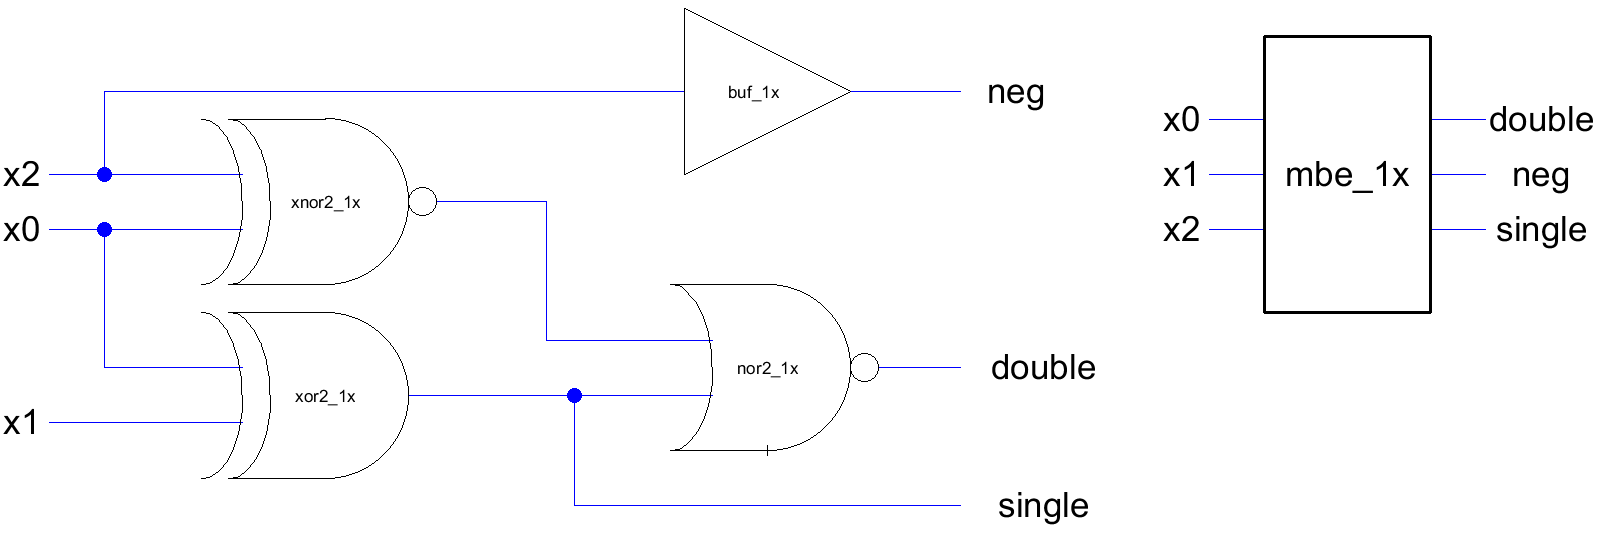
\includegraphics[width=0.43\textwidth]{3.png}
  \centering
  \caption{Encoder Circuit}
  \label{fig:3}
\end{figure}


Since the X vector is 8-bits of size, taking 3 inputs at a time with the repetition of the MSB for each iteration, hence 4 bitslices of the encoder shown above would be needed to realize the logic needed, working in parallel, so delay is the computed for one bitslice only. The layout for that is in Figure \ref{fig:4}.

\begin{figure}[h!]
  \centering
  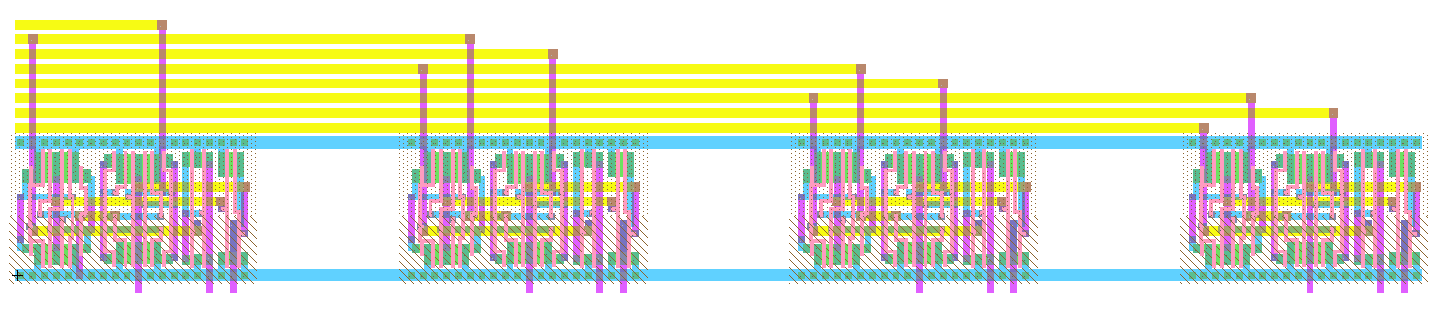
\includegraphics[width=0.48\textwidth]{4.png}
  \centering
  \caption{Encoder Layout}
  \label{fig:4}
\end{figure}



\begin{table}[!h]
%% increase table row spacing, adjust to taste
\renewcommand{\arraystretch}{1.5}
% if using array.sty, it might be a good idea to tweak the value of
% \extrarowheight as needed to properly center the text within the cells
\caption{Encoder - Critical Path Analysis}
\label{tab:t2}
\centering
%% Some packages, such as MDW tools, offer better commands for making tables
%% than the plain LaTeX2e tabular which is used here.
\begin{tabular}{|c|c|}
\hline
~~Critical Path Delay ~~ & ~~2 XORs~~\\
\hline
\end{tabular}
\end{table}


\vspace{-10pt}

\subsection{Partial Products Generator (PPG)}

The PPG is the following part of the circuitry that makes use of the data presented from the encoder signals produced. Consequently, it is the first block that takes in the Y vectors as inputs along with the Double, Single, and Negate signals to be treated, and it hence produces the partial products and sign signals to be used by the following step. The implementation of the PPG in schematic and in layout are shown in Figure \ref{fig:5}.

\begin{table}[!h]
%% increase table row spacing, adjust to taste
\renewcommand{\arraystretch}{1.5}
% if using array.sty, it might be a good idea to tweak the value of
% \extrarowheight as needed to properly center the text within the cells
\caption{PPG - Critical Path Analysis}
\label{tab:t3}
\centering
%% Some packages, such as MDW tools, offer better commands for making tables
%% than the plain LaTeX2e tabular which is used here.
\begin{tabular}{|c|c|}
\hline
~~Critical Path Delay ~~ & 2 NANDs + 1 XOR + 10 NANDs\\
\hline
\end{tabular}
\end{table}

\newpage

\begin{figure}[h!]
  \centering
  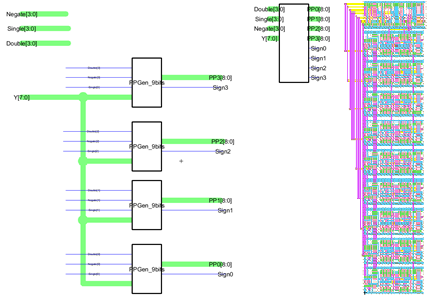
\includegraphics[width=0.4\textwidth]{5.png}
  \centering
  \caption{PPG schematic and layout}
  \label{fig:5}
\end{figure}

\vspace{-10pt}

\subsection{Compressor Tree}

The following part of the logic is the compressor tree, which computes addition using a full adder logic as shown in the bitslice in Figure \ref{fig:6}.

\begin{figure}[h!]
  \centering
  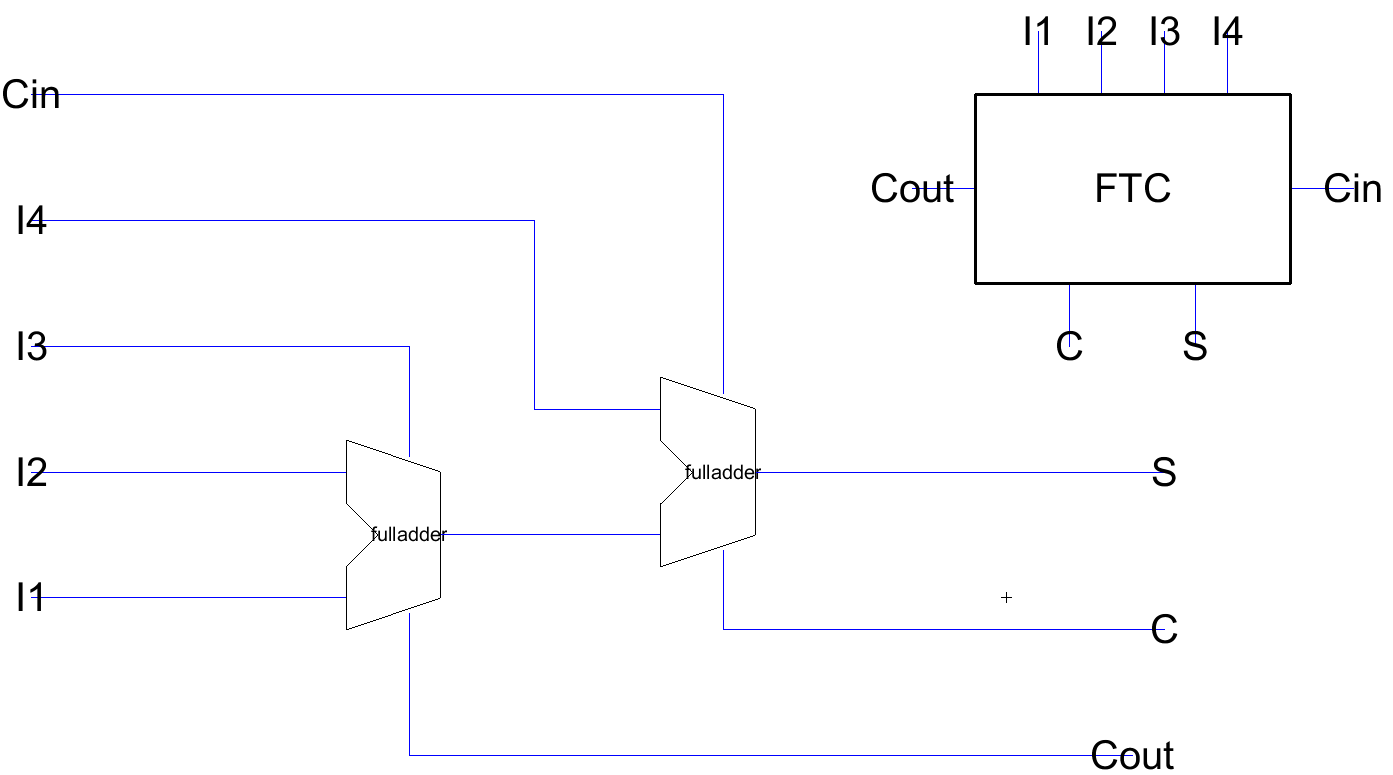
\includegraphics[width=0.4\textwidth]{6.png}
  \centering
  \caption{Four-to-Two Compressor Circuit}
  \label{fig:6}
\end{figure}


The advantage of the tree architecture is that the delay through it is not as high as any other alternative implementation of the architecture, which is evident in the combined design seen in Figure \ref{fig:7}.

\begin{figure}[h!]
  \centering
  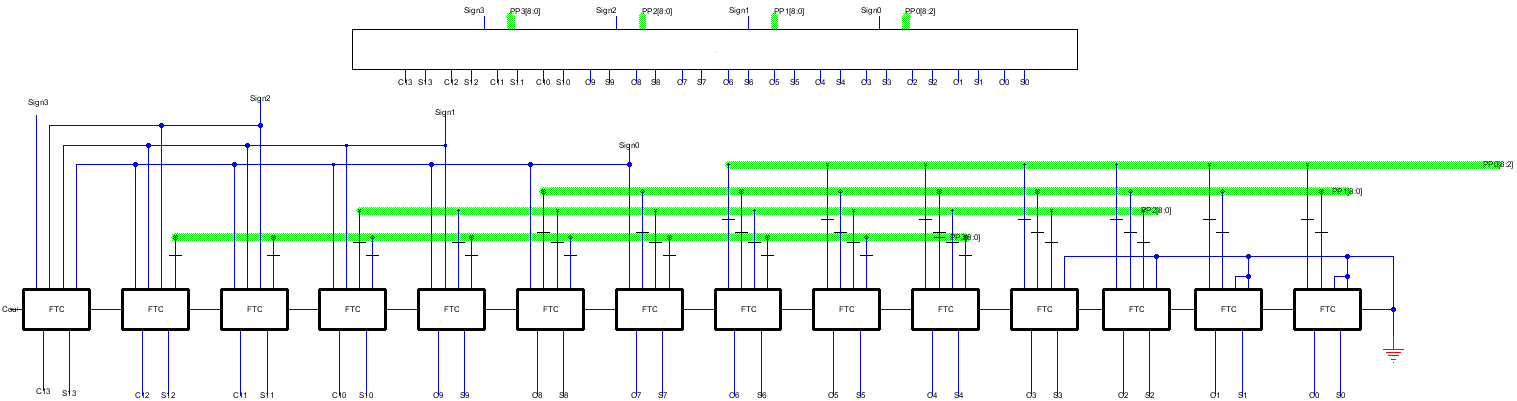
\includegraphics[width=0.45\textwidth]{7.png}
  \centering
  \caption{Compressor Tree Desing}
  \label{fig:7}
\end{figure}


\begin{table}[!h]
%% increase table row spacing, adjust to taste
\renewcommand{\arraystretch}{1.5}
% if using array.sty, it might be a good idea to tweak the value of
% \extrarowheight as needed to properly center the text within the cells
\caption{Compressor Tree - Critical Path Analysis}
\label{tab:t4}
\centering
%% Some packages, such as MDW tools, offer better commands for making tables
%% than the plain LaTeX2e tabular which is used here.
\begin{tabular}{|c|c|}
\hline
~~Critical Path Delay ~~ & 2 XORs\\
\hline
\end{tabular}
\end{table}

\vspace{-10pt}




\subsection{Carry Propagate Adder (CPA)}

This is the final stage that computes the overall value of the product of X and Y. It adds up the outputs of the following stage, with the first block having only 2, hence a half adder was implemented to save up on transistor count.

Exploiting the fact that the critical path delay of the overall design combined comes through the last block of full adder, with that critical delay being larger than that of the CPA adder itself (with a worst case delay assumed for ripple-carry adder), we realize that it is ultimately more beneficial to optimize for transistor count rather than delay. This resulted in designing a ripple-carry adder.

For the full adder blocks, multiple realizations where compared seen in Table 
\ref{tab:t5}.


\begin{table}[!h]
%% increase table row spacing, adjust to taste
\renewcommand{\arraystretch}{1.2}
% if using array.sty, it might be a good idea to tweak the value of
% \extrarowheight as needed to properly center the text within the cells
\caption{Different Full Adders realizations - Comparison}
\label{tab:t5}
\centering
%% Some packages, such as MDW tools, offer better commands for making tables
%% than the plain LaTeX2e tabular which is used here.
\begin{tabular}{| p{1cm} | p{2cm} | p{2cm} | p{2cm} |}
\hline
~~ & \textbf{FA1} & \textbf{FA2} & \textbf{FA3}\\\hline
$S_{out}$ & $A\otimes B\otimes C_{in}$ & $(A\otimes B) \otimes C_{in} $ & 
$\overline{C_{out}}(A+B+C)+ ABC$\\\hline
$C_{out}$ & $AB + A C_{in} + B C_{in}$ & $AB + C_{in}  (A\otimes B) $ & $AB + A C_{in} + B C_{in}$\\\hline
Transistor Count/bit & 32 & 30 & 28\\\hline
\end{tabular}
\end{table}


It is seen that the FA3 design results in the least number of transistors per bit due to exploiting the readily available signal from $\overline{C_{out}}$. Luckily, it is the one available in the given standard library. Transistor level schematic is shown in Figure \ref{fig:8}.

\vspace{-10pt}

\begin{figure}[h!]
  \centering
  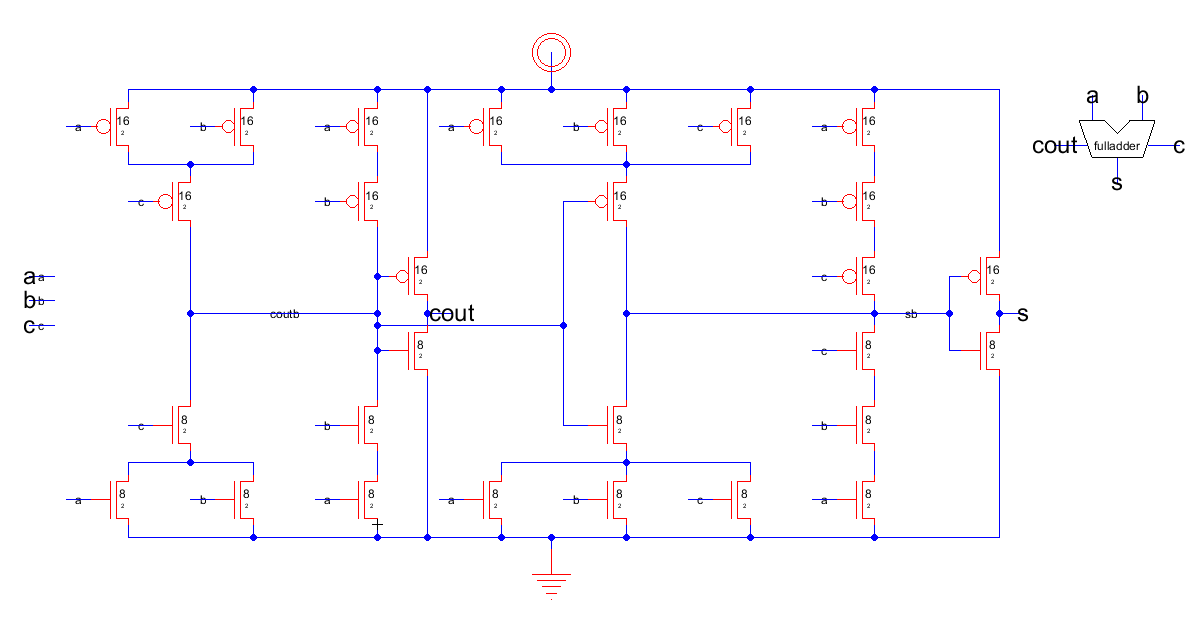
\includegraphics[width=0.4\textwidth]{8.png}
  \centering
  \caption{Full Adder - Transistor level schematic}
  \label{fig:8}
\end{figure}

\vspace{-10pt}

\begin{table}[!h]
%% increase table row spacing, adjust to taste
\renewcommand{\arraystretch}{1.5}
% if using array.sty, it might be a good idea to tweak the value of
% \extrarowheight as needed to properly center the text within the cells
\caption{CPA - Critical Path Analysis}
\label{tab:t6}
\centering
%% Some packages, such as MDW tools, offer better commands for making tables
%% than the plain LaTeX2e tabular which is used here.
\begin{tabular}{|c|c|}
\hline
~~Critical Path Delay : CPA only ~~ & 12 MAJ + 1 AND + 1 XOR\\\hline
~~Critical Path Delay : Through overall ~~ & 1 XOR\\\hline
\end{tabular}
\end{table}

\vspace{-10pt}


\subsection{Whole Design}

\begin{figure}[h!]
  \centering
  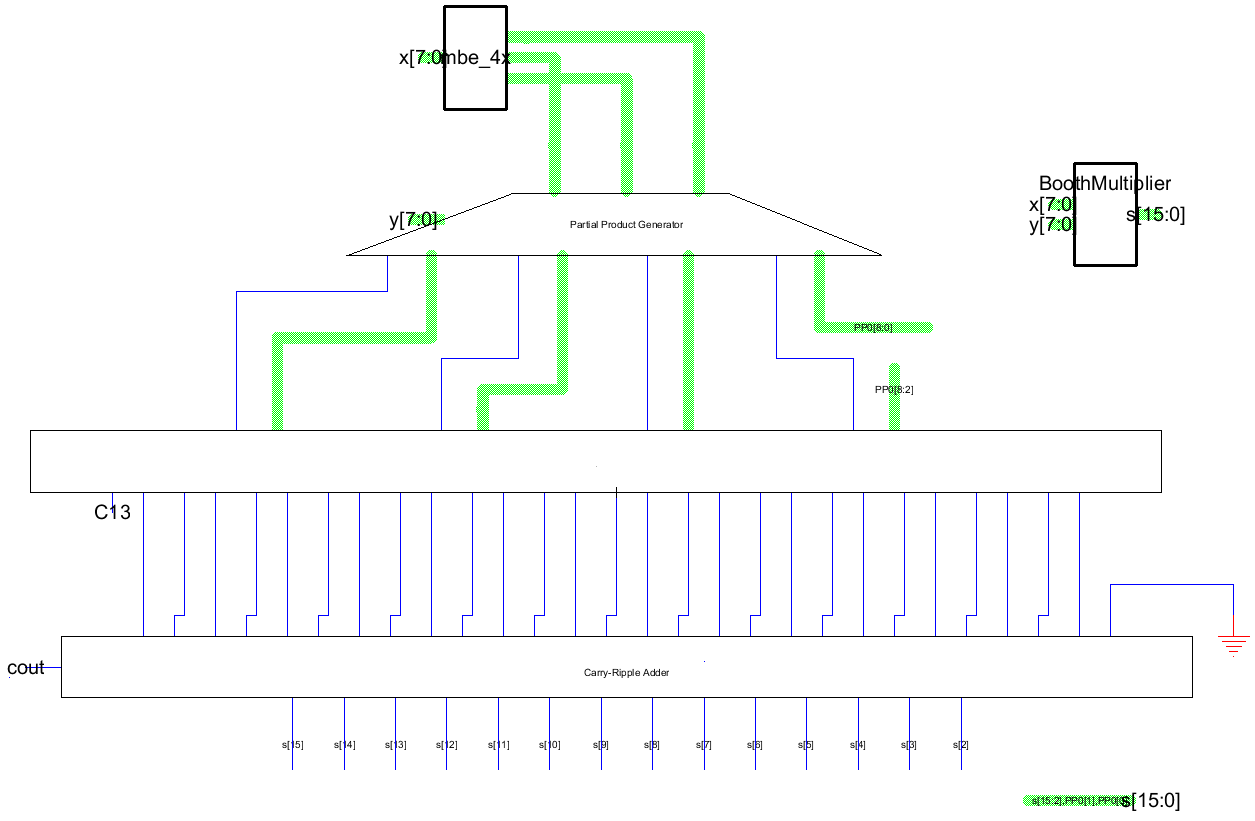
\includegraphics[width=0.3\textwidth]{9.png}
  \centering
  \caption{Whole schematic}
  \label{fig:9}
\end{figure}


The whole design in Figure \ref{fig:9} is the schematic level, while the layout level is shown below as part of the MIPS core to save report space.


\section{MIPS Integration}

In order to integrate the design into the 8-bit MIPS core, modifications to the datapath needed to be implemented along with the Finite State Machine (FSM) to define the states of the processor for the PLA controller. Accordingly, M-type command was introduced and it is defined as follows:


\begin{table}[!h]
%% increase table row spacing, adjust to taste
\renewcommand{\arraystretch}{1.5}
% if using array.sty, it might be a good idea to tweak the value of
% \extrarowheight as needed to properly center the text within the cells
\caption{Extended MIPS ISA: M-type Command}
\label{tab:t7}
\centering
%% Some packages, such as MDW tools, offer better commands for making tables
%% than the plain LaTeX2e tabular which is used here.
\begin{tabular}{|c|c|c|c|c|}
\hline
\textbf{opcode}&\textbf{ra} & \textbf{rb} & \textbf{rd} &\textbf{XX}\\\hline
6 bits & 5 bits & 5 bits & 5 bits & XX\\\hline
\end{tabular}
\end{table}


This new instruction set architecture is what is be used at the assembly level when calling for the multiplier function which would accordingly call on the proper pathway from the modified datapath shown in Figure \ref{fig:10}.

\vspace{-10pt}

\begin{figure}[h!]
  \centering
  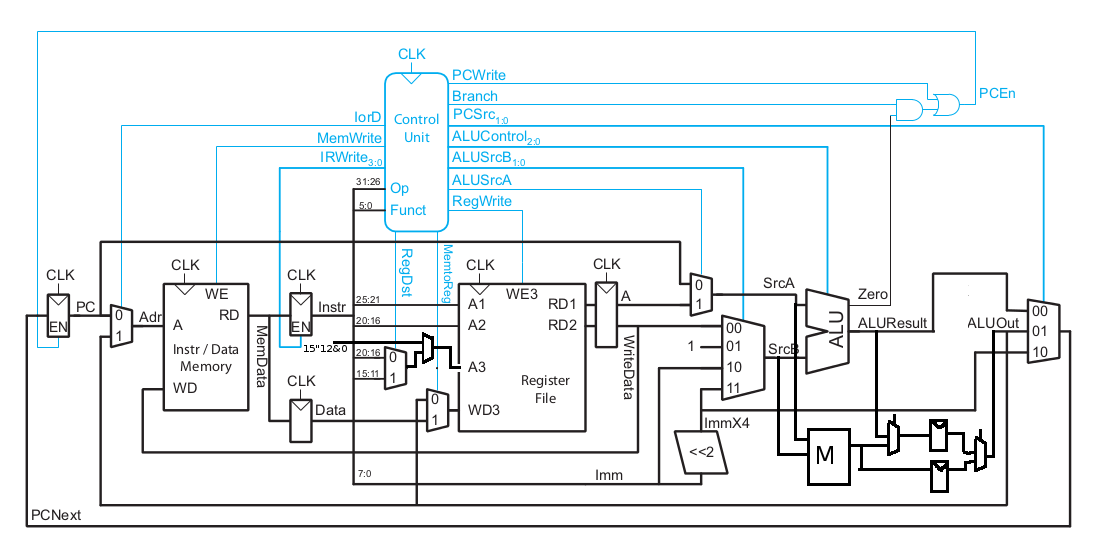
\includegraphics[width=0.45\textwidth]{10.png}
  \centering
  \caption{Modified MIPS datapath}
  \label{fig:10}
\end{figure}


This is then also reflected in modifications for the PLA generator, which is then embedded into the controller. The layout of the entire design is then integrated within the MIPS core, with the ALU shifted to save space for the multiplier as shown in Figure \ref{fig:11}.

\begin{figure}[h!]
  \centering
  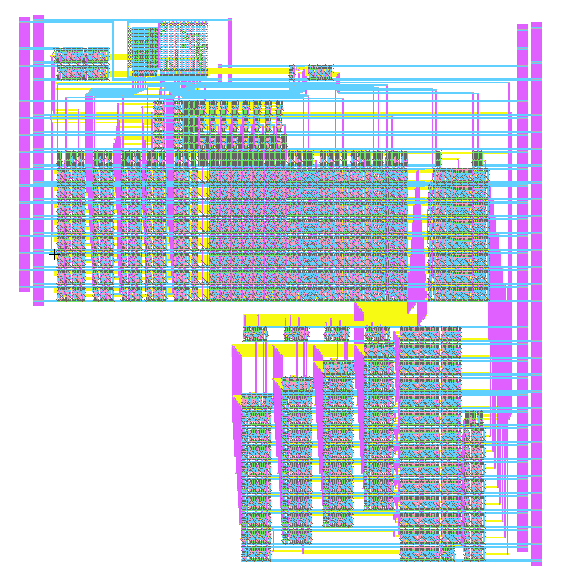
\includegraphics[width=0.4\textwidth]{11.png}
  \centering
  \caption{Entire Desing - Layout}
  \label{fig:11}
\end{figure}


\section{Comparison: Baugh-Wooley Multiplier}

Baugh-Wooley Multiplier (BWM) is the 2’s compliment option for the basic array multiplier. Figure \ref{fig:12} shows the schematic for it.

\vspace{-10pt}

\begin{figure}[h!]
  \centering
  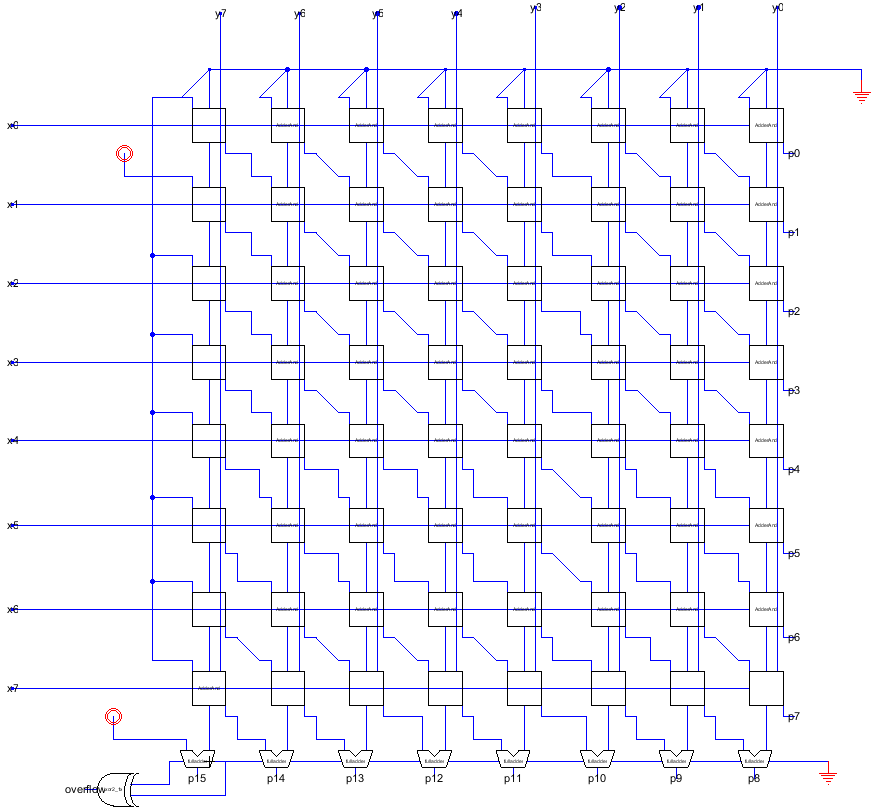
\includegraphics[width=0.45\textwidth]{12.png}
  \centering
  \caption{BWM schematic}
  \label{fig:12}
\end{figure}


The main differences between BWM and the regular array multiplier is that for the blocks on the bottom and left sides, the xi and yi are NANDed instead of ANDed, along with a 2 Vdd connections as shown in the figure instead of ground. Due to regularity and similarity in all blocks, the design demonstrates compactness in the layout level as seen in Figure \ref{fig:13}.

\begin{figure}[h!]
  \centering
  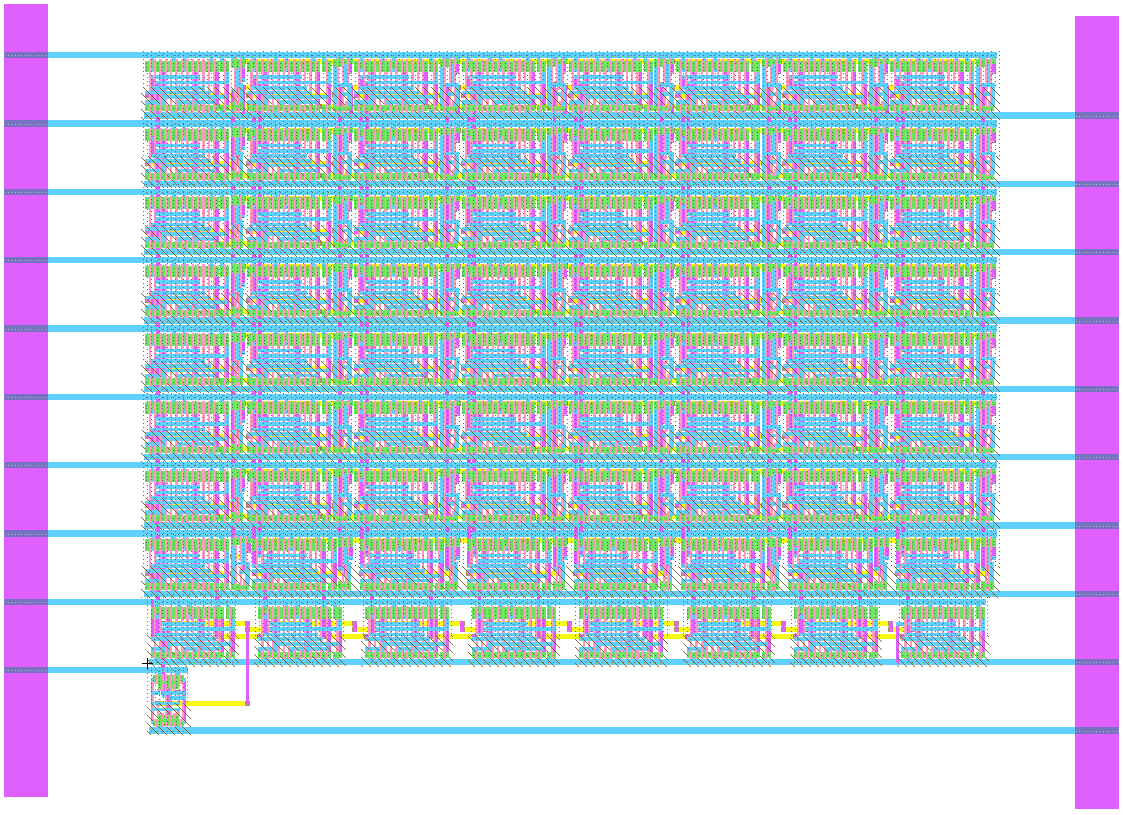
\includegraphics[width=0.45\textwidth]{13.png}
  \centering
  \caption{BWM layout}
  \label{fig:13}
\end{figure}

\vspace{-10pt}

\subsection{8-bit Comparison}

Table \ref{tab:t8} demonstrates that Transistor Count and Area are relatively superior for the BWM, with the Booth Multiplier superior for the Critical Path Delay.

\begin{table}[!h]
%% increase table row spacing, adjust to taste
\renewcommand{\arraystretch}{1.2}
% if using array.sty, it might be a good idea to tweak the value of
% \extrarowheight as needed to properly center the text within the cells
\caption{Modified Booth \& BWM: 8-bit comparison}
\label{tab:t8}
\centering
%% Some packages, such as MDW tools, offer better commands for making tables
%% than the plain LaTeX2e tabular which is used here.
\begin{tabular}{| c | c | c | }
\hline
\textbf{Comparison} & \textbf{Modified Booth} & 
\textbf{BWM} 0\\\hline
Transistor Count & 2886 & 2384\\\hline
Area & $2.4 M \lambda^2$ & $1.3 M \lambda^2$\\\hline
Critical Path Delay & 8 XORs + 10 ANDs + 2 NANDs 
& 8 XORs + 9 ANDs + 8 ORs\\\hline
\end{tabular}
\end{table}


\subsection{16-bit Comparison}

Without designing, the results for the critical path delay for both multipliers were theoretically analyzed and were shown to give the following Table \ref{tab:t9}:

\begin{table}[!h]
%% increase table row spacing, adjust to taste
\renewcommand{\arraystretch}{1.2}
% if using array.sty, it might be a good idea to tweak the value of
% \extrarowheight as needed to properly center the text within the cells
\caption{Modified Booth \& BWM: 16-bit comparison}
\label{tab:t9}
\centering
%% Some packages, such as MDW tools, offer better commands for making tables
%% than the plain LaTeX2e tabular which is used here.
\begin{tabular}{| c | c | c | }
\hline
\textbf{Comparison} & \textbf{Modified Booth} & 
\textbf{BWM} 0\\\hline
Critical Path Delay & 9 XORs + 18 ANDs + 2 NANDs 
& 16 XORs + 17 ANDs + 16 MAJs\\\hline
\end{tabular}
\end{table}


A plot of the total number of gates the process needs to go through vs the number of bits is shown in Figure \ref{fig:14}.

\begin{figure}[h!]
  \centering
  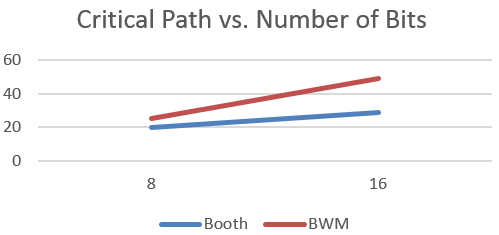
\includegraphics[width=0.4\textwidth]{14.png}
  \centering
  \caption{BWM and Booth Multiplier Comparison: Total Number of gates}
  \label{fig:14}
\end{figure}

\vspace{-5pt}

\section{Evaluation}

Evaluating this, we see that the main strength of the booth multiplier is for the critical path delay it has compared to BWM. This is also a function of the number of bits being used; as they increase, the delay slope for BWM steeps higher than the booth multiplier making the latter more efficient.



\section{Testing}


All designs were passed thorugh an initial testing phase for functionality: Booth multiplier through Quartus and Array Multiplier thorugh a written Verilog code. The final electric products were tested by exporting the Verilog files and testbenching them through ModelSim. The MIPS full design verification was done by MILE, the MIPS emulator. All test vectors were completely exhaustive, covering all 28*28=216 options for the input vectors X and Y.



\begin{thebibliography}{1}


\bibitem{booth} 
A. Booth, \emph{A signed binary multiplication technique}, Quarterly J. 
Mechanics and Applied Mathematics, vol. IV, pt. 2, Jun. 1951, pp. 236-240.

\bibitem{mcs} 
O. MacSorley, \emph{High-Speed arithmetic in binary computers}, Proc. IRE, 
vol. 49, pt. 1, Jan. 1961, pp. 67–91.

\bibitem{cash}
M. Hatamian and G. Cash, \emph{A 70-MHz 8-bit ×8-bit parallel pipelined 
multiplier in 2.5-um CMOS}, 
JSSC, vol. 21, no. 4, Aug. 1986, pp. 505-513.

\bibitem{tb}
Neil Weste and David Harris. \emph{CMOS VLSI Design: A Circuits and 
Systems Perspective}, 4th edition, Addison-Wesley Publishing Company, 
USA.



\end{thebibliography}




% that's all folks
% como estan bitchez
\end{document}

